% =====================================================================
%  SECTION 5 -- THEORETICAL MODEL  (rewritten, self-contained)
%  Coupled magnetic-mechanical oscillator: two copper leaf springs with
%  repelling magnets.
%  Build:  tectonic -X compile theory_section.tex   (or pdflatex x2)
%  Needs fig_release.pdf in the same folder (made by plot in theory_guide).
% =====================================================================
\documentclass[11pt,a4paper]{article}
\usepackage[a4paper,margin=2.4cm]{geometry}
\usepackage[T1]{fontenc}
\usepackage[utf8]{inputenc}
\usepackage{lmodern}
\usepackage{amsmath,amssymb,bm}
\usepackage{booktabs,array}
\usepackage{enumitem}
\usepackage{xcolor}
\usepackage{graphicx}
\usepackage{tikz}
\usetikzlibrary{decorations.pathmorphing,arrows.meta,calc,positioning,patterns}
\usepackage{pgfplots}
\pgfplotsset{compat=1.18}
\usepackage{caption}
\captionsetup{font=small,labelfont=bf,width=0.92\textwidth}
\usepackage{tcolorbox}
\usepackage[hidelinks]{hyperref}

% ---- house style shared with the rest of the essay (Section 1 figures) ----
\colorlet{copper}{orange!80!black}      % leaf springs
\colorlet{clampgray}{gray!60}           % clamps
\colorlet{basegray}{gray!30}            % non-magnetic base
\colorlet{magnetS}{red!70}              % S pole (red)   -- as in Fig. 1 of the essay
\colorlet{magnetN}{blue!70}             % N pole (blue)
% \magnetSN{x}{y}{width}{height} / \magnetNS{...}: two-colour magnet block with its lower-left
%   corner at (x,y); SN / NS is the pole order from left to right (S = red, N = blue, as in
%   Figure 1 of the essay). Pole letters are printed in white.
\newcommand{\magnetSN}[4]{%
  \fill[magnetS] (#1,#2) rectangle ({#1+#3/2},{#2+#4});
  \fill[magnetN] ({#1+#3/2},#2) rectangle ({#1+#3},{#2+#4});
  \node[white,font=\tiny] at ({#1+#3/4},{#2+#4/2}) {S};
  \node[white,font=\tiny] at ({#1+3*#3/4},{#2+#4/2}) {N};}
\newcommand{\magnetNS}[4]{%
  \fill[magnetN] (#1,#2) rectangle ({#1+#3/2},{#2+#4});
  \fill[magnetS] ({#1+#3/2},#2) rectangle ({#1+#3},{#2+#4});
  \node[white,font=\tiny] at ({#1+#3/4},{#2+#4/2}) {N};
  \node[white,font=\tiny] at ({#1+3*#3/4},{#2+#4/2}) {S};}
\newcommand{\muz}{\mu_0}
\newcommand{\mum}{\mu_{\mathrm m}}
\newcommand{\dd}{\mathrm{d}}
\newcommand{\un}[1]{\,\mathrm{#1}}
\newtcolorbox{keybox}{colback=blue!4,colframe=blue!50!black,boxrule=0.6pt,arc=2pt,left=4pt,right=4pt,top=3pt,bottom=3pt}
\newtcolorbox{notebox}{colback=gray!6,colframe=gray!55!black,boxrule=0.5pt,arc=2pt,left=4pt,right=4pt,top=3pt,bottom=3pt,fontupper=\small}

\setcounter{section}{4}   % so that this is Section 5, as in the essay

\begin{document}

\section{Theoretical model}\label{sec:theory}

\noindent\textbf{Notation.} Throughout this section the two springs are numbered 1 (left) and 2 (right). All symbols are collected in Table~\ref{tab:symbols} at the end of the section; each is also defined where it first appears.

\medskip
The model is built in five steps.
\begin{enumerate}[nosep,leftmargin=1.8em]
\item Each leaf spring with its magnet is reduced to a mass $m$ on a spring of stiffness $k$ (Section~\ref{sec:spring}).
\item The repulsive force between the two magnets is written down, treating each magnet as a point magnetic dipole (Section~\ref{sec:force}).
\item The equilibrium of the two springs under this repulsion is described, and the coordinates used for the motion are defined (Section~\ref{sec:equilibrium}).
\item The repulsion is \emph{linearised} about the equilibrium separation; this turns the magnetic force into a second spring of stiffness $\gamma$ joining the two masses (Section~\ref{sec:linearise}).
\item The resulting pair of coupled equations is solved for the two normal modes, giving the relation that the experiment tests, and for the motion after a single spring is released, which is what is actually recorded (Sections~\ref{sec:modes}--\ref{sec:beats}).
\end{enumerate}

% ============================================================================
\subsection{The leaf spring with its magnet as a mass on a spring}\label{sec:spring}

\subsubsection{Geometry and symbols}

Each leaf spring is a thin rectangular copper strip clamped at its lower end and free at its upper end (Figure~\ref{fig:cantilever}). The part of the strip above the clamp has \emph{free length} $L$, \emph{width} $b$ (into the page) and \emph{thickness} $h$ (the small dimension, in the plane of bending). A beam fixed at one end and free at the other is called a \emph{cantilever}. The magnet is glued to the face of the strip at its upper end. When the tip is pushed sideways by a horizontal force $F$ the strip bends and the tip moves horizontally by a distance $x$.

\begin{figure}[!htbp]
\centering
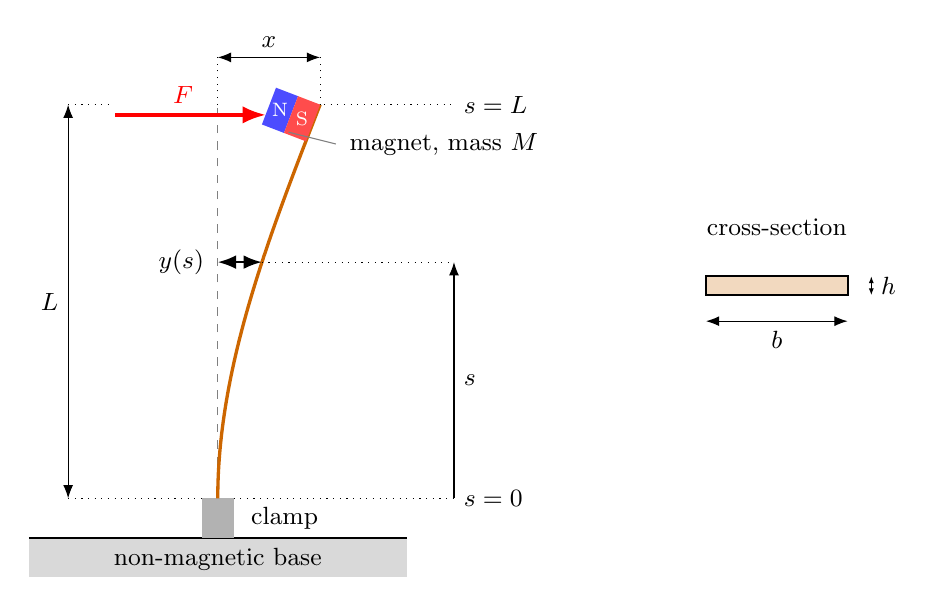
\begin{tikzpicture}[scale=1,>=Latex]
% base and clamp (style of Section 1)
\fill[basegray] (-2.4,-0.5) rectangle (2.4,0);  \draw[thick] (-2.4,0)--(2.4,0);
\node[font=\small] at (0,-0.27) {non-magnetic base};
\fill[clampgray] (-0.2,0) rectangle (0.2,0.5);
\node[font=\small,anchor=west] at (0.3,0.25) {clamp};
% undeflected (dashed) and deflected strip: y = x s^2(3L-s)/(2L^3), L = 5
\draw[dashed,gray] (0,0.5)--(0,5.5);
\draw[very thick,copper,domain=0:5,samples=50,variable=\s] plot ({1.3*\s*\s*(15-\s)/250},{0.5+\s});
% magnet glued to the LEFT face of the strip at the tip (frame tilted with the strip, 21 deg);
% N pole outwards (towards the other magnet), S pole against the strip -- as spring 2 in the setup figure
\begin{scope}[shift={(1.3,5.5)},rotate=-21]
  \fill[magnetN] (-0.6,-0.5) rectangle (-0.3,0.0);
  \fill[magnetS] (-0.3,-0.5) rectangle (0.0,0.0);
  \node[white,font=\scriptsize] at (-0.45,-0.25){N}; \node[white,font=\scriptsize] at (-0.15,-0.25){S};
\end{scope}
\node[font=\small,anchor=west] at (1.55,5.0) {magnet, mass $M$};
\draw[gray,thin] (0.9,5.15)--(1.5,5.0);
% tip force: horizontal, through the centre of the magnet, arrow head touching its outer face
\draw[->,red,very thick] (-1.3,5.37)--(0.61,5.37) node[pos=0.45,above,font=\small]{$F$};
% tip deflection
\draw[<->] (0,6.1)--(1.3,6.1) node[midway,above,font=\small]{$x$};
\draw[dotted] (0,5.5)--(0,6.1); \draw[dotted] (1.3,5.5)--(1.3,6.1);
% free length L
\draw[<->] (-1.9,0.5)--(-1.9,5.5) node[midway,left,font=\small]{$L$};
\draw[dotted] (-1.9,0.5)--(-0.2,0.5); \draw[dotted] (-1.9,5.5)--(-1.35,5.5);
% coordinate s and deflection y(s) at a general point (s = 3: phi = 0.432)
\draw[<->,thick] (0,3.5)--(0.56,3.5); \node[font=\small,anchor=east] at (-0.05,3.5){$y(s)$};
\draw[dotted] (0.56,3.5)--(3.0,3.5);
\draw[->] (3.0,0.5)--(3.0,3.5) node[midway,right,font=\small]{$s$};
\draw[dotted] (0.2,0.5)--(3.0,0.5);
\node[font=\small,anchor=west] at (3.0,0.5){$s=0$};
\draw[dotted] (1.35,5.5)--(3.0,5.5); \node[font=\small,anchor=west] at (3.0,5.5){$s=L$};
% cross-section inset
\begin{scope}[shift={(6.2,3.2)}]
\node[font=\small] at (0.9,0.75) {cross-section};
\draw[thick,fill=copper!25] (0,-0.12) rectangle (1.8,0.12);
\draw[<->] (0,-0.45)--(1.8,-0.45) node[midway,below,font=\small]{$b$};
\draw[{Latex[length=2.5pt]}-{Latex[length=2.5pt]}] (2.1,-0.12) -- (2.1,0.12)
  node[midway, right, font=\small]{$h$};
\end{scope}
\end{tikzpicture}
\caption{Geometry of the leaf spring.}
\label{fig:cantilever}
\end{figure}

\subsubsection{Why a bent strip pushes back: bending moment and curvature}

A straight strip resists being bent because bending stretches the material on the outside of the curve and compresses it on the inside. Consider a short piece of the strip bent into an arc of radius $R$ (Figure~\ref{fig:bending}). A layer of the strip a distance $z$ from the middle surface (the \emph{neutral surface}, which is neither stretched nor compressed) has length $(R+z)\theta$ instead of $R\theta$, so its strain (fractional extension) is
\begin{equation}
\varepsilon(z)=\frac{(R+z)\theta-R\theta}{R\theta}=\frac{z}{R}.
\end{equation}
By Hooke's law for the material, the stress (force per unit area) in that layer is $\sigma(z)=E\varepsilon(z)=Ez/R$, where $E$ is Young's modulus of copper. Tension on one side and compression on the other form a couple: the total turning moment of these internal forces about the neutral surface is
\begin{equation}
\mathcal M=\int\sigma(z)\,z\,\dd A=\frac{E}{R}\int z^2\,\dd A=\frac{EI}{R},\qquad
I\equiv\int z^2\,\dd A=\int_{-h/2}^{h/2}z^2\,b\,\dd z=\frac{bh^3}{12}.
\label{eq:M_EI}
\end{equation}
$I$ is called the \emph{second moment of area} of the cross-section; it is a purely geometrical quantity ($\mathrm{m^4}$) that measures how far the material sits from the neutral surface. The thickness enters as $h^3$: doubling the thickness makes the strip eight times harder to bend, because the outer layers are both further away (larger strain) and have a longer lever arm.

\begin{figure}[htbp]
\centering
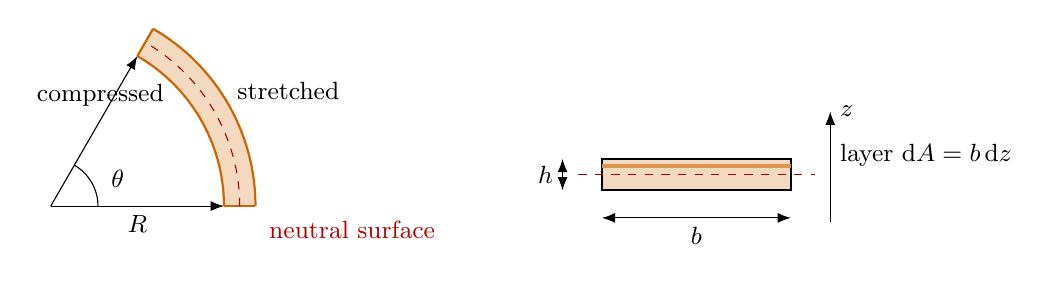
\begin{tikzpicture}[scale=1,>=Latex]
% bent element of the strip
\fill[copper!25] (2.2,0) arc (0:60:2.2) -- ({2.6*cos(60)},{2.6*sin(60)}) arc (60:0:2.6) -- cycle;
\draw[thick,copper] (2.2,0) arc (0:60:2.2);
\draw[thick,copper] (2.6,0) arc (0:60:2.6);
\draw[thick,copper] (2.2,0)--(2.6,0);
\draw[thick,copper] ({2.2*cos(60)},{2.2*sin(60)})--({2.6*cos(60)},{2.6*sin(60)});
\draw[dashed,red!70!black] (2.4,0) arc (0:60:2.4);
\node[red!70!black,anchor=west,font=\small] at (2.65,-0.3) {neutral surface};
\draw[->] (0,0)--(2.2,0) node[midway,below,font=\small]{$R$};
\draw[->] (0,0)--({2.2*cos(60)},{2.2*sin(60)});
\draw (0.6,0) arc (0:60:0.6); \node[font=\small] at (0.85,0.35) {$\theta$};
\node[anchor=west,font=\small] at ({2.65*cos(32)},{2.75*sin(32)}) {stretched};
\node[anchor=east,font=\small] at ({2.1*cos(42)},{2.1*sin(42)}) {compressed};
% cross-section with z
\begin{scope}[shift={(7.0,0.4)}]
\draw[thick,fill=copper!25] (0,-0.2) rectangle (2.4,0.2);
\draw[dashed,red!70!black] (-0.3,0)--(2.7,0);
\fill[copper!70] (0,0.08) rectangle (2.4,0.14);
\draw[->] (2.9,-0.6)--(2.9,0.8) node[right,font=\small]{$z$};
\draw[<->] (-0.5,-0.2)--(-0.5,0.2) node[midway,left,font=\small]{$h$};
\draw[<->] (0,-0.55)--(2.4,-0.55) node[midway,below,font=\small]{$b$};
\node[right,font=\small] at (2.9,0.25) {layer $\dd A=b\,\dd z$};
\end{scope}
\end{tikzpicture}
\caption{Left: a short element of the strip bent to radius of curvature $R$ through angle $\theta$. Layers outside the neutral surface (dashed) are stretched, layers inside are compressed, by a strain $z/R$. Right: the cross-section, with $z$ measured from the neutral surface; a layer of area $\dd A=b\,\dd z$ at height $z$ carries stress $Ez/R$, and the sum of their moments is $EI/R$.}
\label{fig:bending}
\end{figure}

Equation~\eqref{eq:M_EI} is the \emph{bending equation}: to hold a piece of the strip at curvature $1/R$ requires a moment $EI/R$; equivalently, wherever a moment $\mathcal M$ acts, the strip curves with $1/R=\mathcal M/EI$. For small deflections the curvature of the curve $y(s)$ is its second derivative, $1/R\approx y''(s)$ (the exact expression is $y''/(1+y'^2)^{3/2}$, and $y'^2\ll1$ for the deflections used here), so
\begin{equation}
EI\,y''(s)=\mathcal M(s).
\label{eq:curvature}
\end{equation}

\subsubsection{The static deflection curve of a cantilever with a tip force}

Now apply a sideways force $F$ at the tip ($s=L$) and nothing else. (Because the strip is vertical, the weights of the strip and magnet act \emph{along} the strip: they produce no bending moment while it is straight, and only a second-order correction once it is bent, which is neglected. This is one advantage of the vertical arrangement.) Cut the strip mentally at a distance $s$ from the clamp and look at the part above the cut (Figure~\ref{fig:moment}). The only sideways force on that part is $F$, acting at the tip, a distance $L-s$ above the cut. For the part to be in equilibrium the internal moment at the cut must balance the moment of $F$:
\begin{equation}
\mathcal M(s)=F\,(L-s).
\label{eq:Ms}
\end{equation}
The moment is largest at the clamp ($s=0$), where the lever arm is the whole length, and zero at the tip: the strip is bent most sharply near the clamp and is straight at the free end, as Figure~\ref{fig:cantilever} shows.

\begin{figure}[htbp]
\centering
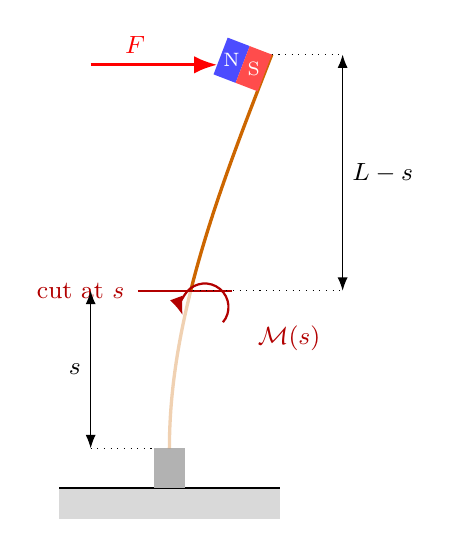
\begin{tikzpicture}[scale=1,>=Latex]
\fill[basegray] (-1.4,-0.4) rectangle (1.4,0); \draw[thick] (-1.4,0)--(1.4,0);
\fill[clampgray] (-0.2,0) rectangle (0.2,0.5);
% strip: part below the cut faint, part above the cut full colour
\draw[very thick,copper,opacity=0.3,domain=0:2,samples=30,variable=\t] plot ({1.3*\t*\t*(15-\t)/250},{0.5+\t});
\draw[very thick,copper,domain=2:5,samples=40,variable=\t] plot ({1.3*\t*\t*(15-\t)/250},{0.5+\t});
% magnet on the left face at the tip, as in Figure 1
\begin{scope}[shift={(1.3,5.5)},rotate=-21]
  \fill[magnetN] (-0.6,-0.5) rectangle (-0.3,0.0);
  \fill[magnetS] (-0.3,-0.5) rectangle (0.0,0.0);
  \node[white,font=\scriptsize] at (-0.45,-0.25){N}; \node[white,font=\scriptsize] at (-0.15,-0.25){S};
\end{scope}
% cut
\draw[thick,red!70!black] (-0.4,2.5)--(0.8,2.5);
\node[red!70!black,anchor=east,font=\small] at (-0.45,2.5) {cut at $s$};
% tip force, arrow head touching the magnet
\draw[->,red,very thick] (-1.0,5.37)--(0.61,5.37) node[pos=0.35,above,font=\small]{$F$};
% lever arm
\draw[<->] (2.2,2.5)--(2.2,5.5) node[midway,right,font=\small]{$L-s$};
\draw[dotted] (0.3,2.5)--(2.2,2.5); \draw[dotted] (1.3,5.5)--(2.2,5.5);
% s
\draw[<->] (-1.0,0.5)--(-1.0,2.5) node[midway,left,font=\small]{$s$};
\draw[dotted] (-1.0,0.5)--(-0.2,0.5);
% internal moment at the cut
\draw[->,thick,red!70!black] (0.68,2.1) arc (-40:200:0.3);
\node[red!70!black,anchor=west,font=\small] at (1.0,1.9) {$\mathcal M(s)$};
\end{tikzpicture}
\caption{Finding the bending moment. The part of the strip above an imaginary cut at height $s$ (full colour, together with the magnet) is acted on by the tip force $F$, with lever arm $L-s$, and by the internal moment $\mathcal M(s)$ exerted on it by the part below the cut (faint). For equilibrium of the upper part, $\mathcal M(s)=F(L-s)$: largest at the clamp, zero at the tip.}
\label{fig:moment}
\end{figure}

Inserting \eqref{eq:Ms} into \eqref{eq:curvature} gives a differential equation for the shape of the strip,
\begin{equation}
EI\,y''(s)=F(L-s),
\end{equation}
which is solved by integrating twice. The two integration constants are fixed by the clamp, which holds the strip at $s=0$ both in position and in direction: $y(0)=0$ and $y'(0)=0$.
\begin{align}
EI\,y'(s)&=F\Big(Ls-\frac{s^2}{2}\Big)+c_1, & y'(0)=0\ \Rightarrow\ c_1&=0,\\
EI\,y(s)&=F\Big(\frac{Ls^2}{2}-\frac{s^3}{6}\Big)+c_2, & y(0)=0\ \Rightarrow\ c_2&=0 .
\end{align}
Hence
\begin{equation}
y(s)=\frac{F}{6EI}\,s^2(3L-s),\qquad\text{and at the tip}\qquad x\equiv y(L)=\frac{F}{6EI}\,L^2\cdot2L=\frac{FL^3}{3EI}.
\label{eq:ys}
\end{equation}
Dividing the shape by the tip deflection gives the \emph{normalised deflection curve}
\begin{equation}
\varphi(s)\equiv\frac{y(s)}{y(L)}=\frac{s^2(3L-s)}{2L^3},\qquad \varphi(0)=0,\quad \varphi(L)=1,
\label{eq:phi}
\end{equation}
which says what fraction of the tip's displacement each point of the strip undergoes: zero at the clamp, $\tfrac{5}{16}\approx0.31$ half-way up, and $1$ at the tip. (The strip is not bent uniformly: the lower half, where the moment is large, does most of the bending.) This curve is used in Section~\ref{sec:meff} to find the effective mass.

\subsubsection{The stiffness $k$}

Equation~\eqref{eq:ys} shows that the tip deflection is proportional to the force. The tip therefore behaves as a linear (Hookean) spring with stiffness
\begin{equation}
\boxed{\;k\equiv\frac{F}{x}=\frac{3EI}{L^3}=\frac{Ebh^3}{4L^3}\;}
\label{eq:k}
\end{equation}
Three checks that the formula is sensible: doubling the free length $L$ makes the spring $2^3=8$ times \emph{softer} (a long strip is floppy); doubling the thickness $h$ makes it $8$ times \emph{stiffer}; doubling the width $b$ only doubles $k$ (like two strips side by side).

\subsubsection{The effective mass $m$}\label{sec:meff}

If the strip were massless the oscillating mass would be the magnet alone, $M$. But the strip has mass too, and it moves; the difficulty is that it does not all move equally. A point at distance $s$ from the clamp moves $\varphi(s)$ times as far as the tip, so during an oscillation it also moves $\varphi(s)$ times as \emph{fast}: the strip near the clamp is almost stationary while the tip moves with the magnet (Figure~\ref{fig:rayleigh}).

\begin{figure}[htbp]
\centering
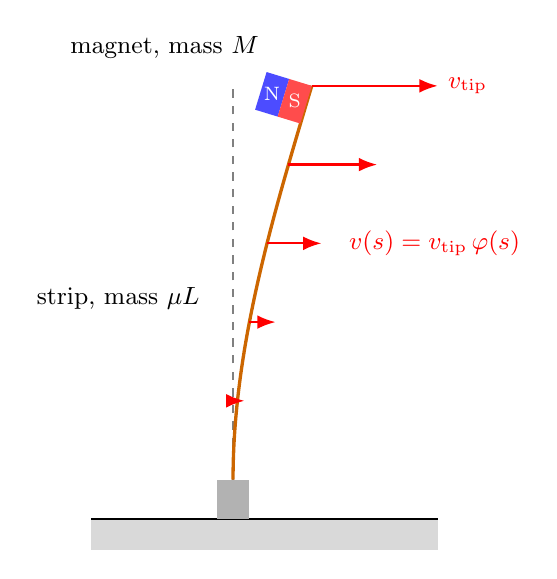
\begin{tikzpicture}[scale=1,>=Latex]
\fill[basegray] (-1.8,-0.4) rectangle (2.6,0); \draw[thick] (-1.8,0)--(2.6,0);
\fill[clampgray] (-0.2,0) rectangle (0.2,0.5);
\draw[dashed,gray] (0,0.5)--(0,5.5);
\draw[very thick,copper,domain=0:5,samples=50,variable=\t] plot ({1.0*\t*\t*(15-\t)/250},{0.5+\t});
% velocity arrows, length proportional to phi(s)
\foreach \t in {1,2,3,4}{
  \pgfmathsetmacro{\v}{1.6*\t*\t*(15-\t)/250}
  \draw[->,red,thick] ({1.0*\t*\t*(15-\t)/250},{0.5+\t}) -- ++({\v},0);
}
% magnet on the left face at the tip (local slope about 17 deg)
\begin{scope}[shift={(1.0,5.5)},rotate=-17]
  \fill[magnetN] (-0.6,-0.5) rectangle (-0.3,0.0);
  \fill[magnetS] (-0.3,-0.5) rectangle (0.0,0.0);
  \node[white,font=\scriptsize] at (-0.45,-0.25){N}; \node[white,font=\scriptsize] at (-0.15,-0.25){S};
\end{scope}
\node[font=\small,anchor=south east] at (0.45,5.72) {magnet, mass $M$};
% tip velocity (magnet and strip tip move together)
\draw[->,red,thick] (1.0,5.5) -- ++(1.6,0) node[right,font=\small]{$v_{\rm tip}$};
\node[red,anchor=west,font=\small] at (1.35,3.5) {$v(s)=v_{\rm tip}\,\varphi(s)$};
\node[font=\small,anchor=east] at (-0.3,2.8) {strip, mass $\mu L$};
\end{tikzpicture}
\caption{Rayleigh's method. During the oscillation every point of the strip is assumed to move in proportion to the static deflection curve $\varphi(s)$ of equation~\eqref{eq:phi}, so its velocity is $v_{\rm tip}\varphi(s)$: nearly zero near the clamp, equal to the magnet's velocity at the tip (arrows). The strip's kinetic energy is the same as that of a point mass $\tfrac{33}{140}\mu L$ moving with the tip.}
\label{fig:rayleigh}
\end{figure}

\emph{Rayleigh's method} turns this into a single number by comparing kinetic energies. Let $\mu$ be the mass per unit length of the strip (so the strip's total mass is $\mu L$). A short piece of strip of length $\dd s$ has mass $\mu\,\dd s$ and speed $v_{\rm tip}\varphi(s)$, so the kinetic energy of the whole strip is
\begin{equation}
K_{\rm strip}=\int_0^L\tfrac12\,\mu\,\big[v_{\rm tip}\varphi(s)\big]^2\dd s
=\tfrac12\Big[\mu\int_0^L\varphi(s)^2\,\dd s\Big]v_{\rm tip}^2 .
\end{equation}
The bracket is the mass of a fictitious point particle that, moving with the tip, would have the same kinetic energy as the strip. With $\varphi$ from \eqref{eq:phi}, writing $u=s/L$,
\begin{equation}
\int_0^L\varphi^2\,\dd s=\frac{L}{4}\int_0^1u^4(3-u)^2\,\dd u
=\frac{L}{4}\int_0^1\big(9u^4-6u^5+u^6\big)\dd u
=\frac{L}{4}\Big(\frac95-1+\frac17\Big)=\frac{L}{4}\cdot\frac{33}{35}=\frac{33}{140}\,L .
\end{equation}
Adding the magnet, the total kinetic energy is $\tfrac12\big(M+\tfrac{33}{140}\mu L\big)v_{\rm tip}^2$, so the system behaves as a single \emph{effective mass}
\begin{equation}
\boxed{\;m=M+\tfrac{33}{140}\,\mu L\approx M+0.24\,\mu L\;}
\label{eq:meff}
\end{equation}
attached to a spring of stiffness $k$. (Strictly, $M$ should include the glue and any holder, and the magnet's own size adds a small rotational term; both are negligible here.) The assumption that the strip keeps its \emph{static} shape while vibrating is an approximation, but a good one: for a bare strip with no tip mass the exact analysis of the fundamental mode gives a coefficient $3/3.516^2=0.243$ in place of $33/140=0.236$, a $3\,\%$ difference in a term that is itself only a fraction of $m$; with a magnet at the tip the true mode shape is even closer to the static tip-load curve. The potential energy of the bent strip is $\tfrac12kx^2$ by \eqref{eq:k}, so a single spring with its magnet is a simple harmonic oscillator with
\begin{equation}
\omega_0^2=\frac{k}{m},\qquad f_0=\frac{1}{2\pi}\sqrt{\frac{k}{m}} .
\label{eq:f0}
\end{equation}

\begin{notebox}
\textbf{Why measure $k$ and $m$ instead of calculating them.} Equations~\eqref{eq:k} and \eqref{eq:meff} explain how the constants arise, but they are not used to compute them: Young's modulus of a rolled copper strip is uncertain by $\sim10\,\%$, and $h^3$ turns a $3\,\%$ uncertainty in thickness into $9\,\%$ in $k$. Instead, (i) plucking each spring with its own magnet mounted and the other magnet removed gives $f_0$ and hence $k/m$ directly, and (ii) a load--deflection graph gives $k$; together they give $m$. The test of the exponent in Section~\ref{sec:main} needs neither, as will be seen.
\end{notebox}

% ============================================================================
\subsection{The force between the two magnets}\label{sec:force}

\subsubsection{A small magnet as a dipole; its field on the axis}

A permanent magnet is equivalent, as far as its external field is concerned, to a small loop of current. Its strength is measured by its \emph{magnetic dipole moment} $\mum$ (unit $\mathrm{A\,m^2}$; for a loop of area $S$ carrying current $I$, $\mum=IS$). The field of a dipole at distances large compared with its size has a standard form; on the dipole's own axis, at distance $r$ from its centre, the field is directed along the axis and has magnitude
\begin{equation}
B(r)=\frac{\muz}{4\pi}\,\frac{2\mum}{r^3},
\label{eq:Baxis}
\end{equation}
where $\muz=4\pi\times10^{-7}\un{T\,m\,A^{-1}}$ is the permeability of free space. (Equation~\eqref{eq:Baxis} follows from the Biot--Savart field on the axis of a current loop of radius $a$, $B=\muz Ia^2/[2(a^2+r^2)^{3/2}]$, in the limit $r\gg a$: $B\to\muz Ia^2/2r^3=\muz(I\pi a^2)/2\pi r^3=\muz\,2\mum/4\pi r^3$.) The essential feature is the \emph{inverse cube}. For a real magnet, $\mum\approx B_{\rm r}V/\muz$, where $B_{\rm r}$ is the remanence quoted by the manufacturer and $V$ the magnet's volume.

\begin{figure}[htbp]
\centering
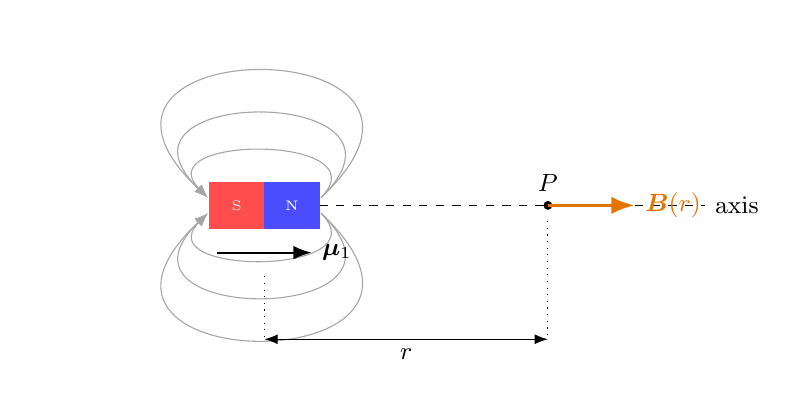
\begin{tikzpicture}[scale=1,>=Latex]
\foreach \r in {1.0,1.7,2.5}{
  \draw[gray!70,->] (0.72,0.1) .. controls (\r+0.5,\r*0.9) and (-\r-0.5,\r*0.9) .. (-0.72,0.1);
  \draw[gray!70,->] (0.72,-0.1) .. controls (\r+0.5,-\r*0.9) and (-\r-0.5,-\r*0.9) .. (-0.72,-0.1);
}
\magnetSN{-0.7}{-0.3}{1.4}{0.6}
\draw[->,thick] (-0.6,-0.6)--(0.6,-0.6) node[right,font=\small]{$\bm\mu_1$};
\draw[dashed] (0.7,0)--(5.6,0) node[right,font=\small]{axis};
\fill (3.6,0) circle (1.6pt); \node[above,font=\small] at (3.6,0.05){$P$};
\draw[->,very thick,orange!90!black] (3.6,0)--(4.7,0) node[right,font=\small]{$\bm B(r)$};
\draw[<->] (0,-1.7)--(3.6,-1.7) node[midway,below,font=\small]{$r$};
\draw[dotted] (0,-0.9)--(0,-1.7); \draw[dotted] (3.6,-0.2)--(3.6,-1.7);
\end{tikzpicture}
\caption{The field of a small magnet (a magnetic dipole of moment $\bm\mu_1$, magnitude $\mum$, pointing from S to N). Grey: field lines. At a point $P$ on the axis, at distance $r$ from the \emph{centre} of the magnet, the field points along the axis in the direction of the moment, with magnitude $\muz2\mum/4\pi r^3$.}
\label{fig:dipole}
\end{figure}

\subsubsection{Energy and force of the second magnet}

Place a second identical magnet on the same axis with its like pole facing the first (Figure~\ref{fig:twomagnets}). A dipole $\bm\mu_2$ in a field $\bm B$ has potential energy
\begin{equation}
U=-\bm\mu_2\cdot\bm B,
\end{equation}
lowest when the moment is parallel to the field (a compass needle aligns with the field). With like poles facing, $\bm\mu_2$ points \emph{against} $\bm B_1$, so the energy is positive:
\begin{equation}
U(r)=+\mum B_1(r)=\frac{\muz}{4\pi}\,\frac{2\mum^2}{r^3}.
\end{equation}
The force on magnet~2 along the axis is minus the derivative of this energy with respect to $r$:
\begin{equation}
\boxed{\;F(r)=-\frac{\dd U}{\dd r}=\frac{\muz}{4\pi}\,\frac{6\mum^2}{r^4}=\frac{3\muz\mum^2}{2\pi\,r^4}\;}
\label{eq:F}
\end{equation}
The sign is positive, i.e.\ the force tends to \emph{increase} $r$: the magnets repel, and by Newton's third law magnet~1 feels an equal force the other way. The force falls as the \emph{fourth} power of the separation because the field falls as $r^{-3}$ and the force is proportional to its gradient.

\begin{figure}[htbp]
\centering
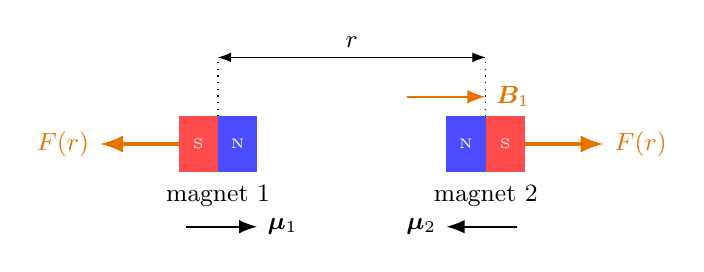
\begin{tikzpicture}[scale=1,>=Latex]
\magnetSN{0}{-0.35}{1.0}{0.7}
\magnetNS{3.4}{-0.35}{1.0}{0.7}
\node[font=\small,below] at (0.5,-0.4){magnet 1}; \node[font=\small,below] at (3.9,-0.4){magnet 2};
\draw[->,thick] (0.1,-1.05)--(1.0,-1.05) node[right,font=\small]{$\bm\mu_1$};
\draw[->,thick] (4.3,-1.05)--(3.4,-1.05) node[left,font=\small]{$\bm\mu_2$};
\draw[->,thick,orange!90!black] (2.9,0.6)--(3.9,0.6) node[right,font=\small]{$\bm B_1$};
\draw[<->] (0.5,1.1)--(3.9,1.1) node[midway,above,font=\small]{$r$};
\draw[dotted] (0.5,0.35)--(0.5,1.1); \draw[dotted] (3.9,0.35)--(3.9,1.1);
\draw[->,very thick,orange!90!black] (4.4,0)--(5.4,0) node[right,font=\small]{$F(r)$};
\draw[->,very thick,orange!90!black] (0,0)--(-1.0,0) node[left,font=\small]{$F(r)$};
\end{tikzpicture}
\caption{Two identical magnets on a common axis with like poles (N) facing. The field $\bm B_1$ of magnet~1 at magnet~2 points to the right; the moment $\bm\mu_2$ of magnet~2 points to the left, so the energy $-\bm\mu_2\cdot\bm B_1$ is positive and decreases with $r$: the magnets repel with $F(r)=3\muz\mum^2/2\pi r^4$, equal and opposite on the two magnets.}
\label{fig:twomagnets}
\end{figure}

\begin{notebox}
\textbf{Two remarks on $F(r)$.} (i) The $r$ in \eqref{eq:F} is the distance between the \emph{centres} of the magnets, not the gap between their faces; this is why the separation $d$ is defined centre-to-centre throughout the essay ($d=\text{gap}+\text{thickness}$ for two equal magnets). (ii) The dipole formula is exact only in the limit $r\gg D$ ($D$ = magnet diameter). Here $r/D$ is only of order $2$--$6$, so deviations are expected at the smallest separations; this is assumption~(a) below and is examined in the evaluation.
\end{notebox}

% ============================================================================
\subsection{Equilibrium and coordinates}\label{sec:equilibrium}

With both magnets mounted the repulsion pushes the two tips apart until each spring's restoring force balances it (Figure~\ref{fig:equilibrium}). If the tips end up a distance $d$ apart (centre to centre), each spring is bent outwards by a static deflection $\delta$ obeying
\begin{equation}
k\,\delta=F(d).
\label{eq:static}
\end{equation}
If the clamps were set a distance $d_0$ apart, then $d=d_0+2\delta$; finding $d$ from $d_0$ would require solving $k(d-d_0)/2=3\muz\mum^2/2\pi d^4$, a fifth-degree equation containing two constants that are not accurately known. The essay avoids this by \emph{measuring} $d$ directly in the equilibrium state, with both magnets mounted and the springs already bent.

From here on:
\begin{itemize}[nosep,leftmargin=1.8em]
\item $x_1$ and $x_2$ are the horizontal displacements of magnets 1 and 2 from their \emph{equilibrium} positions, both counted positive in the same direction (to the right in Figure~\ref{fig:equilibrium});
\item the instantaneous centre-to-centre separation is $r=d+x_2-x_1$ (if magnet~2 moves right and magnet~1 stays, the gap grows);
\item the \emph{unstressed} (straight) position of spring~1 lies $\delta$ to the right of its equilibrium (spring~1 is bent to the left), and that of spring~2 lies $\delta$ to the left of its equilibrium. This is needed for the spring forces in Section~\ref{sec:linearise}.
\end{itemize}

\begin{figure}[htbp]
\centering
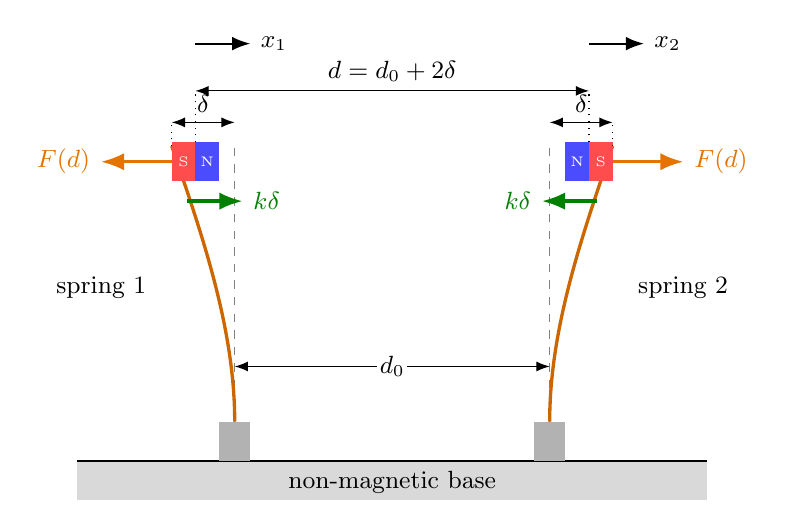
\begin{tikzpicture}[scale=1,>=Latex]
\fill[basegray] (-4.0,-0.5) rectangle (4.0,0); \draw[thick] (-4.0,0)--(4.0,0);
\node[font=\small] at (0,-0.27) {non-magnetic base};
\foreach \sx in {-1,1}{
  \fill[clampgray] ({\sx*2.0-0.2},0) rectangle ({\sx*2.0+0.2},0.5);
  \draw[dashed,gray] ({\sx*2.0},0.5)--({\sx*2.0},4.0);
  \draw[very thick,copper,domain=0:3.5,samples=40,variable=\s]
        plot ({\sx*2.0+\sx*0.8*\s*\s*(10.5-\s)/85.75},{0.5+\s});
}
% magnets glued to the inner faces of the strips (tips at x = -2.8 and +2.8), N poles facing
\magnetSN{-2.8}{3.55}{0.6}{0.5}
\magnetNS{2.2}{3.55}{0.6}{0.5}
\node[font=\small,anchor=east] at (-3.0,2.2) {spring 1}; \node[font=\small,anchor=west] at (3.0,2.2) {spring 2};
% clamp spacing and centre-to-centre separation
\draw[<->] (-2.0,1.2)--(2.0,1.2) node[midway,fill=white,inner sep=1pt,font=\small]{$d_0$};
\draw[<->] (-2.5,4.7)--(2.5,4.7) node[midway,above,font=\small]{$d=d_0+2\delta$};
\draw[dotted] (-2.5,4.05)--(-2.5,4.7); \draw[dotted] (2.5,4.05)--(2.5,4.7);
% static deflection delta
\draw[<->] (2.0,4.3)--(2.8,4.3) node[midway,above,font=\small]{$\delta$};
\draw[<->] (-2.8,4.3)--(-2.0,4.3) node[midway,above,font=\small]{$\delta$};
\draw[dotted] (2.8,4.0)--(2.8,4.3); \draw[dotted] (-2.8,4.0)--(-2.8,4.3);
% forces on each tip: repulsion outwards, elastic restoring force inwards
\draw[->,very thick,orange!90!black] (2.8,3.8)--(3.7,3.8) node[right,font=\small]{$F(d)$};
\draw[->,very thick,orange!90!black] (-2.8,3.8)--(-3.7,3.8) node[left,font=\small]{$F(d)$};
\draw[->,very thick,green!50!black] (2.6,3.3)--(1.9,3.3) node[left,font=\small]{$k\delta$};
\draw[->,very thick,green!50!black] (-2.6,3.3)--(-1.9,3.3) node[right,font=\small]{$k\delta$};
% displacement coordinates
\draw[->,thick] (-2.5,5.3)--(-1.8,5.3) node[right,font=\small]{$x_1$};
\draw[->,thick] (2.5,5.3)--(3.2,5.3) node[right,font=\small]{$x_2$};
\end{tikzpicture}
\caption{Equilibrium with both magnets mounted. The repulsion $F(d)$ bends each spring outwards by $\delta$ from its straight (dashed) position until the elastic restoring force $k\delta$ balances it. The centre-to-centre separation $d$ is defined and measured in this state ($d_0$ is the spacing of the clamps). The displacements $x_1$, $x_2$ used in the equations of motion are measured from these equilibrium positions, both positive to the right.}
\label{fig:equilibrium}
\end{figure}

% ============================================================================
\subsection{Linearising the repulsion: the magnetic ``spring'' $\gamma$}\label{sec:linearise}

During the motion the separation is $r=d+u$ with $u=x_2-x_1$ the change of separation. Since the amplitudes are small compared with $d$, the force can be replaced by the first two terms of its Taylor series about $r=d$ (geometrically: the curve $F(r)$ is replaced by its tangent at $r=d$, Figure~\ref{fig:linearise}):
\begin{equation}
F(d+u)\approx F(d)+F'(d)\,u
\qquad\Longleftrightarrow\qquad
F(d+u)-F(d)\approx-\gamma\,u,\qquad \gamma\equiv-F'(d).
\label{eq:taylor}
\end{equation}
Differentiating \eqref{eq:F} with $\dd(r^{-4})/\dd r=-4r^{-5}$,
\begin{equation}
\boxed{\;\gamma=-\frac{\dd F}{\dd r}\bigg|_{r=d}=\frac{4F(d)}{d}=\frac{6\muz\mum^2}{\pi\,d^5}\;}
\label{eq:gamma}
\end{equation}
$\gamma$ is the \emph{magnetic stiffness}: the change in the repulsive force per unit change of separation. It is positive because a repulsion that weakens with distance always pushes the magnets back towards their equilibrium separation---if they come closer the push apart grows, if they move apart it weakens and the springs win. So, for small motions, the magnetic field between the magnets behaves exactly like a compressed spring of stiffness $\gamma$ connecting them. This is the crucial step for the exponent: the force goes as $d^{-4}$, but the frequencies will turn out to depend on the \emph{stiffness}, which is the derivative of the force and goes as $d^{-5}$.

\begin{figure}[htbp]
\centering
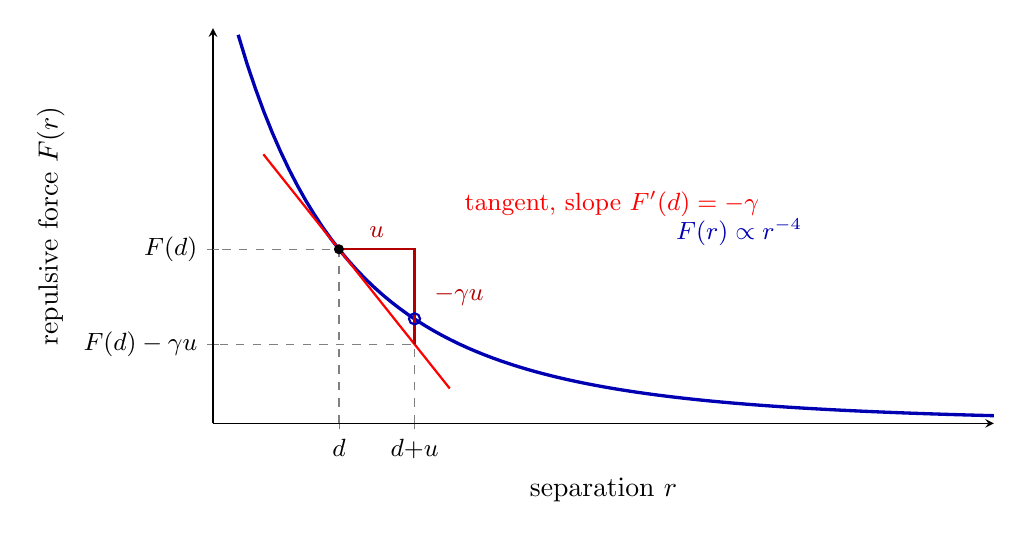
\begin{tikzpicture}
% d = 1.1, u = 0.15:  F(d)=1/1.1^4=0.683,  F'(d)=-4/1.1^5=-2.4837,
% tangent at d+u: 0.683-0.3726=0.310,  true F(1.25)=0.410
\begin{axis}[width=11.5cm,height=6.6cm,axis lines=left,
  xlabel={separation $r$},ylabel={repulsive force $F(r)$},
  xmin=0.85,xmax=2.4,ymin=0,ymax=1.55,
  xtick={1.1,1.25},xticklabels={$d$,$d{+}u$},xticklabel style={font=\small},
  ytick={0.683,0.310},yticklabels={$F(d)$,$F(d)-\gamma u$},yticklabel style={font=\small},
  clip=false]
\addplot[very thick,blue!70!black,domain=0.9:2.4,samples=90]{1/x^4};
\node[blue!70!black,anchor=west,font=\small] at (axis cs:1.75,0.75){$F(r)\propto r^{-4}$};
\addplot[red,thick,domain=0.95:1.32]{0.683-2.4837*(x-1.1)};
\node[red,anchor=west,font=\small] at (axis cs:1.33,0.86){tangent, slope $F'(d)=-\gamma$};
\draw[dashed,gray] (axis cs:1.1,0)--(axis cs:1.1,0.683)--(axis cs:0.85,0.683);
\draw[dashed,gray] (axis cs:1.25,0)--(axis cs:1.25,0.310)--(axis cs:0.85,0.310);
\draw[red!70!black,thick] (axis cs:1.1,0.683)--(axis cs:1.25,0.683)--(axis cs:1.25,0.310);
\node[red!70!black,above,font=\small] at (axis cs:1.175,0.69){$u$};
\node[red!70!black,anchor=west,font=\small] at (axis cs:1.27,0.50){$-\gamma u$};
\addplot[only marks,mark=*,mark size=1.6pt,black] coordinates{(1.1,0.683)};
\addplot[only marks,mark=o,mark size=2pt,blue!70!black,thick] coordinates{(1.25,0.410)};
\end{axis}
\end{tikzpicture}
\caption{Linearisation of the force law. Near the equilibrium separation $d$ the curve $F(r)$ is replaced by its tangent, whose slope is $-\gamma$. Increasing the separation by $u$ reduces the repulsion by $\gamma u$; decreasing it increases the repulsion by the same amount---the behaviour of a compressed spring of stiffness $\gamma$. The gap between the tangent and the true curve (open circle) is the error of the approximation; it grows with $u/d$ and is discussed in the evaluation.}
\label{fig:linearise}
\end{figure}

% ============================================================================
\subsection{Equations of motion and normal modes}\label{sec:modes}

\subsubsection{Newton's second law for each magnet}

Figure~\ref{fig:fbd} shows the horizontal forces on each magnet when both are displaced. Consider magnet~1. Its displacement from the \emph{unstressed} position of spring~1 is $x_1-\delta$ (Section~\ref{sec:equilibrium}), so the spring exerts $-k(x_1-\delta)$. The magnetic force on it is $-F(r)$: it is pushed away from magnet~2, i.e.\ in the negative direction, with the magnitude evaluated at the current separation $r=d+u$. Newton's second law, with the effective mass $m$ of \eqref{eq:meff}:
\begin{align}
m\ddot x_1&=-k(x_1-\delta)-F(d+u)\notag\\
          &=-kx_1+\underbrace{k\delta}_{=F(d)\ \text{by \eqref{eq:static}}}-F(d+u)
           =-kx_1+\big[F(d)-F(d+u)\big]\approx-kx_1+\gamma u ,
\label{eq:newton1}
\end{align}
where the last step used \eqref{eq:taylor}. Two things happened here. The constant part of the magnetic force, $F(d)$, was exactly cancelled by the static bend $k\delta$: that is what ``measured from equilibrium'' buys. Only the \emph{change} of the magnetic force survives, and it is proportional to the change of separation $u=x_2-x_1$.

Magnet~2 is the mirror image: its spring force is $-k(x_2+\delta)$ (its unstressed position is $\delta$ to the \emph{left}), the magnetic force on it is $+F(d+u)$, and $k\delta=F(d)$ again cancels the constant part, leaving $m\ddot x_2=-kx_2-\gamma u$. Together:
\begin{equation}
\boxed{\;m\ddot x_1=-kx_1+\gamma(x_2-x_1),\qquad m\ddot x_2=-kx_2-\gamma(x_2-x_1)\;}
\label{eq:eom}
\end{equation}

\begin{figure}[htbp]
\centering
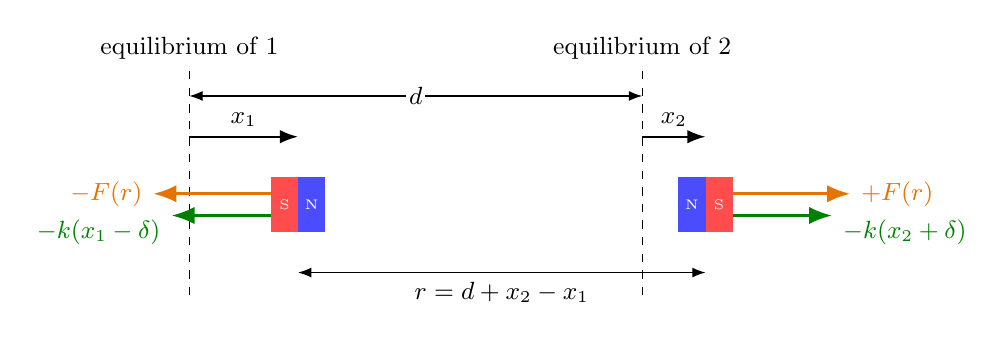
\begin{tikzpicture}[scale=1.15,>=Latex]
\draw[dashed] (0,-1.0)--(0,1.5); \draw[dashed] (5,-1.0)--(5,1.5);
\node[above,font=\small] at (0,1.5){equilibrium of 1}; \node[above,font=\small] at (5,1.5){equilibrium of 2};
\magnetSN{0.9}{-0.3}{0.6}{0.6}
\magnetNS{5.4}{-0.3}{0.6}{0.6}
\draw[->,thick] (0,0.75)--(1.2,0.75) node[midway,above,font=\small]{$x_1$};
\draw[->,thick] (5,0.75)--(5.7,0.75) node[midway,above,font=\small]{$x_2$};
\draw[<->] (1.2,-0.75)--(5.7,-0.75) node[midway,below,font=\small]{$r=d+x_2-x_1$};
\draw[<->] (0,1.2)--(5,1.2) node[midway,fill=white,inner sep=1pt,font=\small]{$d$};
\draw[->,very thick,orange!90!black] (0.9,0.12)--(-0.4,0.12) node[left,font=\small]{$-F(r)$};
\draw[->,very thick,green!50!black] (0.9,-0.12)--(-0.2,-0.12) node[left,font=\small,yshift=-6pt]{$-k(x_1-\delta)$};
\draw[->,very thick,orange!90!black] (6.0,0.12)--(7.3,0.12) node[right,font=\small]{$+F(r)$};
\draw[->,very thick,green!50!black] (6.0,-0.12)--(7.1,-0.12) node[right,font=\small,yshift=-6pt]{$-k(x_2+\delta)$};
\end{tikzpicture}
\caption{Free-body diagram of the two magnets (horizontal forces only, seen from above; orange: magnetic, green: elastic), both shown displaced to the right of their equilibrium positions. Each spring force is proportional to the displacement from that spring's \emph{unstressed} position ($+\delta$ for spring~1, $-\delta$ for spring~2, Figure~\ref{fig:equilibrium}). The magnetic force has magnitude $F(r)$ at the \emph{current} separation and pushes the magnets apart.}
\label{fig:fbd}
\end{figure}

Equations~\eqref{eq:eom} are exactly those of two equal masses on equal springs $k$ joined by a third spring of stiffness $\gamma$ (Figure~\ref{fig:threesprings}): the middle spring exerts $+\gamma(x_2-x_1)$ on the left mass and $-\gamma(x_2-x_1)$ on the right one. The magnetic field has become that third spring.

\begin{figure}[htbp]
\centering
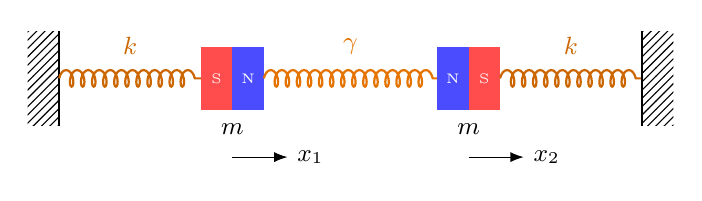
\begin{tikzpicture}[scale=1,>=Latex]
\fill[pattern=north east lines] (-0.4,-0.6) rectangle (0,0.6); \draw[thick](0,-0.6)--(0,0.6);
\draw[decorate,decoration={coil,aspect=0.5,segment length=4pt,amplitude=3pt},copper,thick] (0,0)--(1.8,0) node[midway,above=5pt,font=\small]{$k$};
\magnetSN{1.8}{-0.4}{0.8}{0.8}
\draw[decorate,decoration={coil,aspect=0.5,segment length=4pt,amplitude=3pt},orange!90!black,thick] (2.6,0)--(4.8,0) node[midway,above=5pt,font=\small]{$\gamma$};
\magnetNS{4.8}{-0.4}{0.8}{0.8}
\draw[decorate,decoration={coil,aspect=0.5,segment length=4pt,amplitude=3pt},copper,thick] (5.6,0)--(7.4,0) node[midway,above=5pt,font=\small]{$k$};
\fill[pattern=north east lines] (7.4,-0.6) rectangle (7.8,0.6); \draw[thick](7.4,-0.6)--(7.4,0.6);
\node[font=\small,below] at (2.2,-0.45){$m$}; \node[font=\small,below] at (5.2,-0.45){$m$};
\draw[->] (2.2,-1.0)--(2.9,-1.0) node[right,font=\small]{$x_1$};
\draw[->] (5.2,-1.0)--(5.9,-1.0) node[right,font=\small]{$x_2$};
\end{tikzpicture}
\caption{Mechanical equivalent of equations~\eqref{eq:eom}: two equal masses $m$ on equal springs $k$ (copper: the leaf springs), coupled by a spring of stiffness $\gamma$ (orange: the magnetic repulsion). The picture is schematic; in the apparatus the coupling ``spring'' is the field between the magnets.}
\label{fig:threesprings}
\end{figure}

\begin{notebox}
\textbf{A common slip.} The magnetic term is $\gamma(x_2-x_1)$, not $-\gamma x_1$. The repulsion depends on the \emph{separation} of the magnets, not on where magnet~1 happens to be: if both magnets move together the separation does not change and the magnetic force does not change at all.
\end{notebox}

\subsubsection{Decoupling: the normal coordinates}

The two equations \eqref{eq:eom} are coupled (each contains both $x_1$ and $x_2$), but they can be separated by adding and subtracting them. Adding, the coupling terms cancel:
\begin{equation}
m(\ddot x_1+\ddot x_2)=-k(x_1+x_2)\quad\Longrightarrow\quad m\ddot\eta=-k\,\eta,\qquad \eta\equiv x_1+x_2 .
\end{equation}
Subtracting, the coupling terms add:
\begin{equation}
m(\ddot x_1-\ddot x_2)=-k(x_1-x_2)+2\gamma(x_2-x_1)=-(k+2\gamma)(x_1-x_2)
\ \Longrightarrow\ m\ddot\xi=-(k+2\gamma)\,\xi,\quad \xi\equiv x_1-x_2 .
\end{equation}
$\eta$ and $\xi$ are the \emph{normal coordinates}. Each obeys the simple-harmonic equation $\ddot q=-\omega^2q$ on its own, with
\begin{equation}
\boxed{\;\omega_1^2=\frac{k}{m}\quad(\eta,\ \text{in-phase}),\qquad \omega_2^2=\frac{k+2\gamma}{m}\quad(\xi,\ \text{anti-phase})\;}
\label{eq:modes}
\end{equation}
A motion in which only $\eta$ is non-zero has $\xi=0$, i.e.\ $x_1=x_2$: the two magnets move together, keeping their separation, at angular frequency $\omega_1$ (Figure~\ref{fig:modes}, left). A motion with only $\xi$ non-zero has $x_1=-x_2$: the magnets move in opposite directions, alternately approaching and receding, at $\omega_2$ (right). These two patterns are the \emph{normal modes}: if the system is started exactly in one of them it stays in it, oscillating at a single frequency. Every other motion is a mixture of the two (Section~\ref{sec:beats}).

\begin{figure}[htbp]
\centering
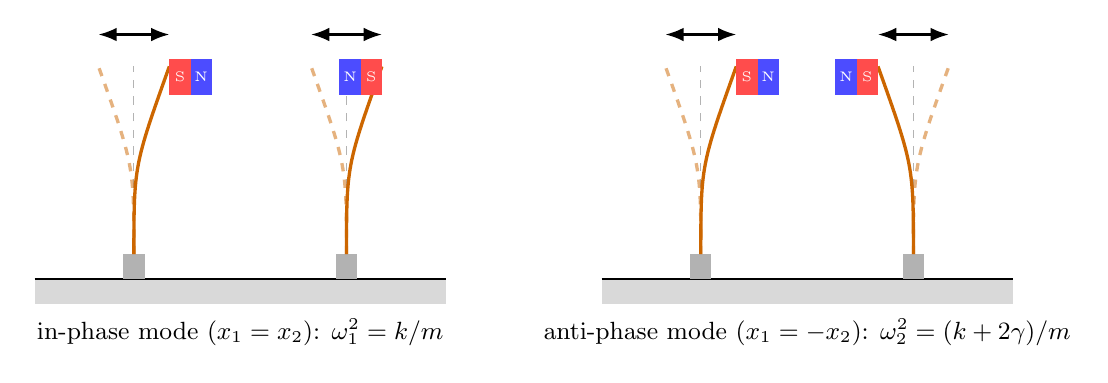
\begin{tikzpicture}[scale=0.9,>=Latex]
\foreach \dx/\lab/\sA/\sB in {0/{in-phase mode ($x_1=x_2$): $\omega_1^2=k/m$}/1/1, 8.0/{anti-phase mode ($x_1=-x_2$): $\omega_2^2=(k+2\gamma)/m$}/1/-1}{
 \begin{scope}[shift={(\dx,0)}]
  \fill[basegray] (-2.9,-0.35) rectangle (2.9,0); \draw[thick] (-2.9,0)--(2.9,0);
  \foreach \sx in {-1,1}{ \fill[clampgray] ({\sx*1.5-0.15},0) rectangle ({\sx*1.5+0.15},0.35); \draw[dashed,gray,opacity=0.6] ({\sx*1.5},0.35)--({\sx*1.5},3.0); }
  % the two extremes of the swing: solid and dashed (same one-control-point curves as in Section 1)
  \draw[very thick,copper] (-1.5,0.35) .. controls (-1.5,1.6) .. ({-1.5+0.5*\sA},3.0);
  \draw[very thick,copper,dashed,opacity=0.5] (-1.5,0.35) .. controls (-1.5,1.6) .. ({-1.5-0.5*\sA},3.0);
  \draw[very thick,copper] (1.5,0.35) .. controls (1.5,1.6) .. ({1.5+0.5*\sB},3.0);
  \draw[very thick,copper,dashed,opacity=0.5] (1.5,0.35) .. controls (1.5,1.6) .. ({1.5-0.5*\sB},3.0);
  % magnets on the inner faces at the solid extreme
  \magnetSN{-1.5+0.5*\sA}{2.6}{0.6}{0.5}
  \magnetNS{1.5+0.5*\sB-0.6}{2.6}{0.6}{0.5}
  \draw[<->,thick] ({-1.5-0.5},3.45)--({-1.5+0.5},3.45);
  \draw[<->,thick] ({1.5-0.5},3.45)--({1.5+0.5},3.45);
  \node[font=\small] at (0,-0.75) {\lab};
 \end{scope}
}
\end{tikzpicture}
\caption{The two normal modes (solid: one extreme of the swing; dashed: the other; magnets drawn at the solid extreme). Left, in-phase: the magnets keep their separation, the magnetic force never changes from its equilibrium value, and each spring oscillates as if alone, at $\omega_1=\sqrt{k/m}$. Right, anti-phase: when each magnet moves $a$ towards the other the separation shrinks by $2a$, so each magnet feels an extra restoring force $\gamma\cdot2a$ on top of $ka$; the effective stiffness is $k+2\gamma$.}
\label{fig:modes}
\end{figure}

The factor 2 in $\omega_2^2$ has a simple origin, visible in Figure~\ref{fig:modes}: in the anti-phase mode a displacement $a$ of each magnet changes the separation by $2a$, so the magnetic spring, which responds to the separation, exerts $2\gamma a$ on each magnet while the magnet itself has moved only $a$. Equivalently, in matrix form $m\ddot{\bm x}=-\mathsf K\bm x$ with $\mathsf K=\begin{pmatrix}k+\gamma&-\gamma\\-\gamma&k+\gamma\end{pmatrix}$, whose eigenvalues are $k$ and $k+2\gamma$ with eigenvectors $(1,1)$ and $(1,-1)$.

Two limits confirm the result. As $d\to\infty$, $\gamma\to0$ and both frequencies become $\sqrt{k/m}$: two uncoupled springs. As $d$ decreases, $\gamma$ grows as $d^{-5}$, $\omega_2$ rises steeply while $\omega_1$ does not move. The size of the coupling can be read from the data: $2\gamma/k=\omega_2^2/\omega_1^2-1=(f_2/f_1)^2-1$, which is $0.67$ at $d=21\un{mm}$ (the magnetic spring is about one third as stiff as a leaf spring) and $0.02$ at $40\un{mm}$.

% ============================================================================
\subsection{The relation tested in this essay}\label{sec:main}

With $\omega=2\pi f$, subtracting the two results of \eqref{eq:modes} eliminates $k$ entirely:
\begin{equation}
\boxed{\;f_2^2-f_1^2=\frac{\omega_2^2-\omega_1^2}{4\pi^2}=\frac{2\gamma}{4\pi^2m}=\frac{\gamma}{2\pi^2m}
=\frac{3\muz\mum^2}{\pi^3m}\;d^{-5}\equiv C\,d^{-5}\;}
\label{eq:main}
\end{equation}
(the last step inserts $\gamma$ from \eqref{eq:gamma}: $6/(2\pi^2\cdot\pi)=3/\pi^3$). Taking natural logarithms,
\begin{equation}
\ln\big(f_2^2-f_1^2\big)=\ln C-5\ln d ,
\label{eq:lnln}
\end{equation}
so a graph of $\ln(f_2^2-f_1^2)$ against $\ln d$ should be a straight line of gradient $-5$ and intercept $\ln C$. The gradient tests the \emph{form} of the force law ($F\propto r^{-4}$ $\Rightarrow$ gradient $-5$); the intercept tests its \emph{magnitude}, and requires $\mum$ and $m$.

\begin{figure}[htbp]
\centering
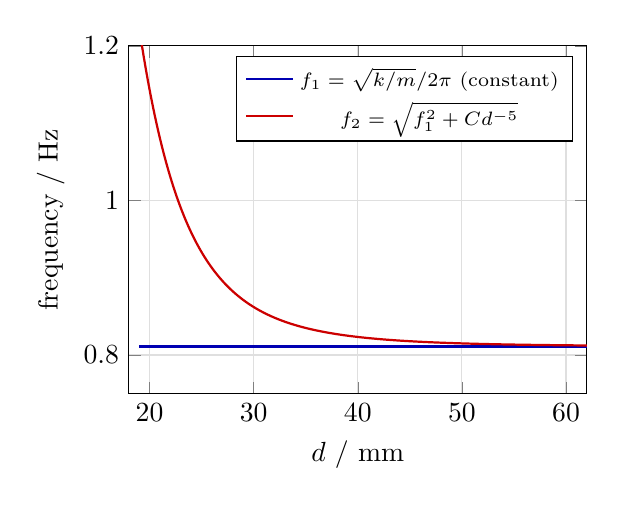
\begin{tikzpicture}
\begin{axis}[width=7.4cm,height=6cm,xlabel={$d$ / mm},ylabel={frequency / Hz},xmin=18,xmax=62,ymin=0.75,ymax=1.2,legend pos=north east,legend style={font=\scriptsize},grid=major,grid style={gray!25}]
\addplot[thick,blue!70!black,domain=19:62,samples=100]{0.811};
\addlegendentry{$f_1=\sqrt{k/m}/2\pi$ (constant)}
\addplot[thick,red!80!black,domain=19:62,samples=200]{sqrt(0.6577+2.08e6/x^5)};
\addlegendentry{$f_2=\sqrt{f_1^2+Cd^{-5}}$}
\end{axis}
\end{tikzpicture}\hfill
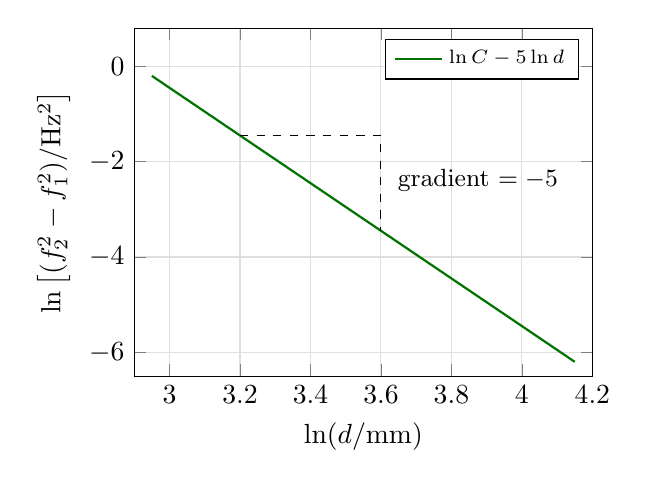
\begin{tikzpicture}
\begin{axis}[width=7.4cm,height=6cm,xlabel={$\ln(d/\mathrm{mm})$},ylabel={$\ln\big[(f_2^2-f_1^2)/\mathrm{Hz^2}\big]$},xmin=2.9,xmax=4.2,ymin=-6.5,ymax=0.8,grid=major,grid style={gray!25},legend pos=north east,legend style={font=\scriptsize}]
\addplot[thick,green!45!black,domain=2.95:4.15]{14.55-5*x};
\addlegendentry{$\ln C-5\ln d$}
\draw[dashed] (axis cs:3.2,-1.45)--(axis cs:3.6,-1.45)--(axis cs:3.6,-3.45);
\node[anchor=west] at (axis cs:3.62,-2.4){\small gradient $=-5$};
\end{axis}
\end{tikzpicture}
\caption{The prediction of the model, drawn with $f_1=0.811\un{Hz}$ and the value of $C$ obtained from the data. Left: $f_1$ is independent of $d$ while $f_2$ falls towards it. Right: the coupling term $f_2^2-f_1^2$ on logarithmic axes is a straight line of gradient exactly $-5$.}
\label{fig:prediction}
\end{figure}

\begin{notebox}
\textbf{Why $f_2^2-f_1^2$ and not simply $f_2$?} (i) $k$ cancels, so the spring constant, Young's modulus and the strip dimensions are not needed to test the force law. (ii) $f_1$ is measured in the \emph{same} record as $f_2$, so a slow drift of the springs (temperature, clamp creep) affects both and largely cancels. (iii) The result is linear in $\gamma$, so the exponent of $d$ appears directly as the gradient of a straight line.

\textbf{Units.} $[\muz\mum^2]=\mathrm{T\,m\,A^{-1}\cdot A^2\,m^4}=\mathrm{T\,A\,m^5}$ and $1\un{T}=1\un{kg\,A^{-1}s^{-2}}$, so $[\muz\mum^2]=\mathrm{kg\,m^5\,s^{-2}}$. Dividing by $m$ (kg) and $d^5$ ($\mathrm{m^5}$) leaves $\mathrm{s^{-2}}$, the units of $f^2$. $C$ has units $\mathrm{m^5\,s^{-2}}$.

\textbf{Static deflection.} From \eqref{eq:static}, \eqref{eq:gamma} and \eqref{eq:main}, $\delta=F(d)/k=\gamma d/4k=\pi^2(f_2^2-f_1^2)\,d/2\omega_1^2$: about $1.8\un{mm}$ at $21\un{mm}$ and $0.1\un{mm}$ at $40\un{mm}$---small compared with $d$, but comparable to the uncertainty in $d$, which is one more reason to measure $d$ at equilibrium.
\end{notebox}

% ============================================================================
\subsection{Motion after releasing one spring: beats}\label{sec:beats}

\subsubsection{The general motion and the mode amplitudes}

Because $\eta$ and $\xi$ each perform simple harmonic motion, the most general motion is
\begin{equation}
\eta(t)=\eta_0\cos(\omega_1t+\phi_1),\qquad \xi(t)=\xi_0\cos(\omega_2t+\phi_2),
\end{equation}
with four constants fixed by the four initial conditions (two positions, two velocities). The frequencies are properties of the system; the \emph{amounts} $\eta_0$, $\xi_0$ of each mode depend only on how the motion is started. In the experiment both springs are released from rest, $\dot x_1(0)=\dot x_2(0)=0$, hence $\dot\eta(0)=\dot\xi(0)=0$, which forces $\phi_1=\phi_2=0$. The mode amplitudes are then simply the initial values of the normal coordinates:
\begin{equation}
\eta_0=x_1(0)+x_2(0),\qquad \xi_0=x_1(0)-x_2(0).
\label{eq:amps}
\end{equation}
Transforming back with $x_1=(\eta+\xi)/2$ and $x_2=(\eta-\xi)/2$:
\begin{equation}
\boxed{\;x_1(t)=\frac{\eta_0}{2}\cos\omega_1t+\frac{\xi_0}{2}\cos\omega_2t,\qquad
x_2(t)=\frac{\eta_0}{2}\cos\omega_1t-\frac{\xi_0}{2}\cos\omega_2t\;}
\label{eq:solution}
\end{equation}
Each spring's displacement is the sum of \emph{two cosines}, one at each mode frequency. Table~\ref{tab:start} lists what different starting conditions produce.

\begin{table}[htbp]
\centering\small
\caption{Mode amplitudes for different ways of starting the motion (both springs released from rest).}
\label{tab:start}
\begin{tabular}{@{}p{4.0cm}ccp{5.6cm}@{}}
\toprule
how the motion is started & $x_1(0),\ x_2(0)$ & $\eta_0,\ \xi_0$ & resulting motion\\
\midrule
both displaced the same way & $A,\ A$ & $2A,\ 0$ & pure in-phase mode: single frequency $f_1$\\
displaced in opposite directions & $A,\ -A$ & $0,\ 2A$ & pure anti-phase mode: single frequency $f_2$\\
spring 1 displaced, spring 2 exactly at equilibrium & $A,\ 0$ & $A,\ A$ & both modes, equal amplitude: beats whose minima reach zero\\
spring 1 \emph{held} at $A$; spring 2 has shifted to $x_{20}$ & $A,\ x_{20}$ & $A+x_{20},\ A-x_{20}$ & both modes, unequal amplitude: beats whose minima do not reach zero\\
\bottomrule
\end{tabular}
\end{table}

\subsubsection{What the Fourier spectrum shows, and why the two peaks are not equal}

A Fourier transform of a record reports the amplitude of the cosine present at each frequency. By \eqref{eq:solution} the record $x_1(t)$ contains exactly two cosines, so its spectrum shows two peaks, at $f_1$ and $f_2$, and (for a record long enough to separate them) their heights are proportional to $\eta_0/2$ and $\xi_0/2$:
\begin{equation}
\frac{\text{height of the peak at }f_2}{\text{height of the peak at }f_1}=\frac{\xi_0}{\eta_0}.
\label{eq:ratio}
\end{equation}
Two consequences are important for the method. First, the \emph{positions} of the peaks, $f_1$ and $f_2$, do not depend on the starting condition at all: a single FFT of a single spring gives both mode frequencies however the spring was released, provided both modes are present. Second, the \emph{heights} depend only on the starting condition, and are equal only in the idealised case $x_2(0)=0$.

That ideal case is not what happens in practice. Spring~1 is \emph{held} at $x_1=A$ for a moment before it is released, and while it is held the repulsion on spring~2 differs from its equilibrium value, so spring~2 shifts to a new rest position before the release. Setting $\ddot x_2=0$ in the second of \eqref{eq:eom} with $x_1=A$:
\begin{equation}
0=-kx_{20}-\gamma(x_{20}-A)\qquad\Longrightarrow\qquad x_{20}=\frac{\gamma}{k+\gamma}\,A ,
\end{equation}
in the same direction as $A$ (spring~2 is pushed away if spring~1 is pushed towards it, and follows if spring~1 is pulled away). By \eqref{eq:amps} and \eqref{eq:ratio},
\begin{equation}
\boxed{\;\frac{\text{height at }f_2}{\text{height at }f_1}=\frac{A-x_{20}}{A+x_{20}}=\frac{k}{k+2\gamma}=\frac{\omega_1^2}{\omega_2^2}=\Big(\frac{f_1}{f_2}\Big)^2\;}
\label{eq:heights}
\end{equation}
With the frequencies measured at $d=23\un{mm}$ ($f_1=0.802$, $f_2=0.996\un{Hz}$) this predicts a ratio of $0.65$; the observed ratio is about $0.6$. The residual difference is of the size expected from the non-linearity of the force at $A=10\un{mm}$ (evaluation). The same shift explains why the beat minima are not zero: the amplitude of $x_1$ swings between $(\eta_0+\xi_0)/2=A$ and $(\eta_0-\xi_0)/2=x_{20}$, so minimum/maximum $=\gamma/(k+\gamma)\approx0.2$ (Figure~\ref{fig:release}). Neither effect moves $f_1$ or $f_2$.

\begin{figure}[htbp]
\centering

\includegraphics[width=\textwidth]{fig_release.pdf}
\caption{The same system ($f_1=0.802$, $f_2=0.996\un{Hz}$; linear model, $A=8\un{mm}$) started in two ways; left: $x_1(t)$ with its envelope, right: its amplitude spectrum, with the predicted peak heights $\eta_0/2$ and $\xi_0/2$ marked. Top: idealised instantaneous release with $x_2(0)=0$---equal mode amplitudes, equal FFT peaks, beat minima at zero. Bottom: hold-and-release, $x_2(0)=A\gamma/(k+\gamma)=1.7\un{mm}$---peak ratio $(f_1/f_2)^2=0.65$ and beat minima of $1.7\un{mm}$. The peak \emph{positions} are identical in both cases. (Generated by \texttt{make\_fig\_release.py}.)}
\label{fig:release}
\end{figure}

\subsubsection{Why two cosines make beats}

Represent each cosine as the horizontal projection of a rotating arrow (Figure~\ref{fig:phasor}): arrow~1 of length $\eta_0/2$ turning at $f_1$ revolutions per second, arrow~2 of length $\xi_0/2$ turning at $f_2$ revolutions per second; $x_1$ is the horizontal projection of their vector sum. Since arrow~2 turns slightly faster, the angle between them grows steadily, by $f_2-f_1$ revolutions per second. When the arrows are aligned the sum is long, $(\eta_0+\xi_0)/2$; half a relative revolution later they oppose and the sum is short, $|\eta_0-\xi_0|/2$; after one full relative revolution they are aligned again. So the \emph{amplitude} of the fast oscillation swells and shrinks with period
\begin{equation}
\boxed{\;T_{\rm beat}=\frac{1}{f_2-f_1},\qquad f_{\rm beat}\equiv\frac{1}{T_{\rm beat}}=f_2-f_1\;}
\label{eq:Tbeat}
\end{equation}
whatever the two lengths are; the lengths only decide how deep the minima go. Meanwhile the sum-arrow itself turns at approximately the mean rate, so the fast oscillation has frequency close to $f_{\rm avg}=(f_1+f_2)/2$ (exactly so for equal lengths).

\begin{figure}[htbp]
\centering
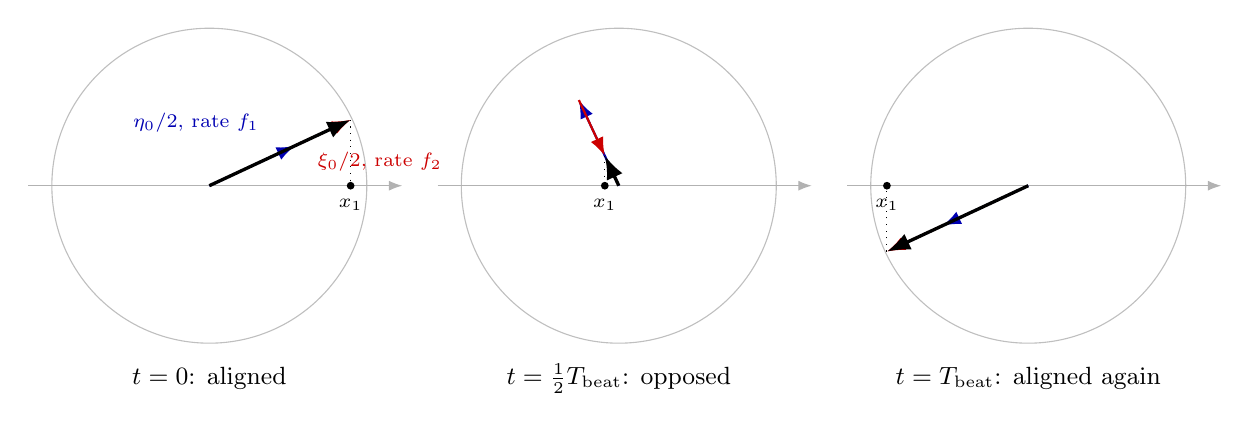
\begin{tikzpicture}[scale=1.0,>=Latex]
\foreach \dx/\ta/\tb/\capA in {0/25/25/{$t=0$: aligned},
                               5.2/115/295/{$t=\tfrac12T_{\rm beat}$: opposed},
                               10.4/205/205/{$t=T_{\rm beat}$: aligned again}}{
 \begin{scope}[shift={(\dx,0)}]
  \draw[gray!50] (0,0) circle (2.0);
  \draw[gray!60,->] (-2.3,0)--(2.45,0);
  \draw[->,thick,blue!70!black] (0,0)--(\ta:1.2) coordinate (p);
  \draw[->,thick,red!80!black] (p)--++(\tb:0.78) coordinate (q);
  \draw[->,very thick,black] (0,0)--(q);
  \draw[dotted] (q)--(q|-0,0);
  \fill (q|-0,0) circle (1.4pt);
  \node[below,font=\scriptsize] at ($(q|-0,0)+(0,-0.05)$) {$x_1$};
  \node[font=\small] at (0,-2.45) {\capA};
 \end{scope}
}
\node[blue!70!black,font=\scriptsize,anchor=south east] at (0.75,0.55) {$\eta_0/2$, rate $f_1$};
\node[red!80!black,font=\scriptsize,anchor=north west] at (1.25,0.55) {$\xi_0/2$, rate $f_2$};
\end{tikzpicture}
\caption{Beats as rotating arrows (phasors). Blue: length $\eta_0/2$, turning at $f_1$ revolutions per second. Red, drawn head-to-tail: length $\xi_0/2$, turning at $f_2$. Black: their sum; $x_1$ is its horizontal projection. The relative angle grows by one full turn every $1/(f_2-f_1)$ seconds, so the length of the black arrow---the amplitude of the fast oscillation---swings between $(\eta_0+\xi_0)/2$ and $|\eta_0-\xi_0|/2$ with exactly that period. Drawn for $\xi_0/\eta_0=0.65$, the hold-and-release case: the amplitude never falls to zero.}
\label{fig:phasor}
\end{figure}

For the equal-amplitude case $\eta_0=\xi_0=A$ the same result follows from the identity $\cos\alpha+\cos\beta=2\cos\frac{\alpha-\beta}{2}\cos\frac{\alpha+\beta}{2}$ with $\alpha=2\pi f_1t$, $\beta=2\pi f_2t$:
\begin{equation}
\boxed{\;x_1(t)=A\cos\!\big(\pi(f_2-f_1)\,t\big)\,\cos\!\big(2\pi f_{\rm avg}\,t\big),\qquad f_{\rm avg}=\frac{f_1+f_2}{2}\;}
\label{eq:beats}
\end{equation}
a fast oscillation at the average frequency whose amplitude $A\cos(\pi(f_2-f_1)t)$ varies slowly (Figure~\ref{fig:beatplot}). The envelope cosine has frequency $(f_2-f_1)/2$, but what is observed is its \emph{modulus}, which has two maxima per cycle; the swellings therefore recur every $1/(f_2-f_1)$, in agreement with \eqref{eq:Tbeat}. Multiplying out $(f_2-f_1)(f_2+f_1)$ gives the link to the coupling term:
\begin{equation}
\boxed{\;f_2^2-f_1^2=2\,f_{\rm beat}\,f_{\rm avg}\;}
\label{eq:beats_identity}
\end{equation}
The beat frequency is the mode splitting itself, and the quantity tested in \eqref{eq:main} is the product of the splitting and twice the average frequency.

\begin{figure}[htbp]
\centering
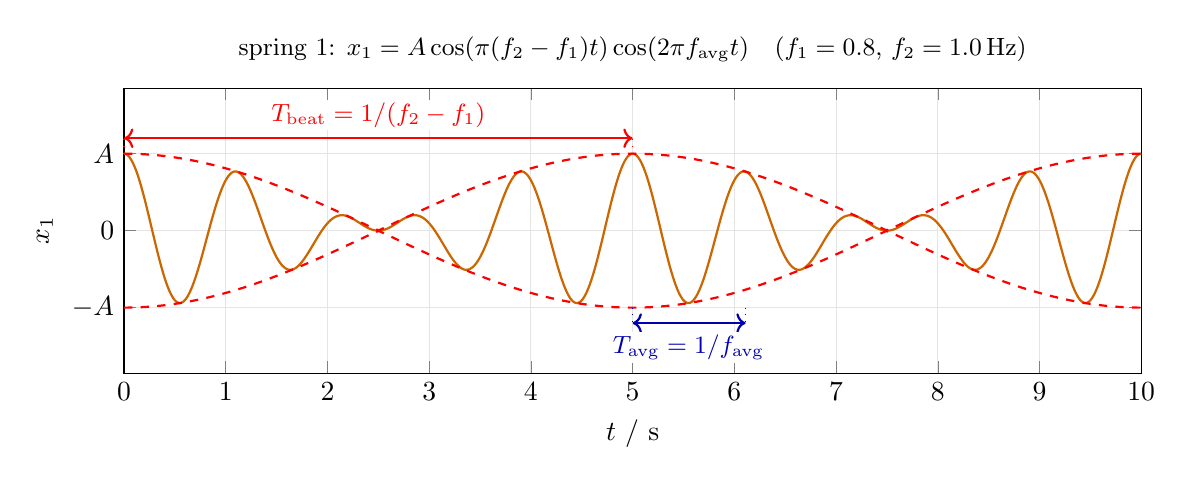
\begin{tikzpicture}
\begin{axis}[width=14.5cm,height=5.2cm,xlabel={$t$ / s},ylabel={$x_1$},xmin=0,xmax=10,ymin=-1.85,ymax=1.85,ytick={-1,0,1},yticklabels={$-A$,$0$,$A$},grid=major,grid style={gray!20},clip=false,title={\small spring 1: $x_1=A\cos(\pi(f_2-f_1)t)\cos(2\pi f_{\rm avg}t)$\quad ($f_1=0.8$, $f_2=1.0\un{Hz}$)}]
\addplot[thick,copper,domain=0:10,samples=700]{cos(deg(0.2*pi*x))*cos(deg(1.8*pi*x))};
\addplot[thick,red,dashed,domain=0:10,samples=300]{abs(cos(deg(0.2*pi*x)))};
\addplot[thick,red,dashed,domain=0:10,samples=300]{-abs(cos(deg(0.2*pi*x)))};
\draw[dotted,red] (axis cs:0,1)--(axis cs:0,1.25); \draw[dotted,red] (axis cs:5,1)--(axis cs:5,1.25);
\draw[<->,thick,red] (axis cs:0,1.2)--(axis cs:5,1.2);
\node[red,fill=white,inner sep=1pt] at (axis cs:2.5,1.5){\small $T_{\rm beat}=1/(f_2-f_1)$};
\draw[dotted,blue!70!black] (axis cs:5,-1)--(axis cs:5,-1.25); \draw[dotted,blue!70!black] (axis cs:6.111,-1)--(axis cs:6.111,-1.25);
\draw[<->,thick,blue!70!black] (axis cs:5,-1.2)--(axis cs:6.111,-1.2);
\node[blue!70!black,fill=white,inner sep=1pt] at (axis cs:5.55,-1.52){\small $T_{\rm avg}=1/f_{\rm avg}$};
\end{axis}
\end{tikzpicture}\\
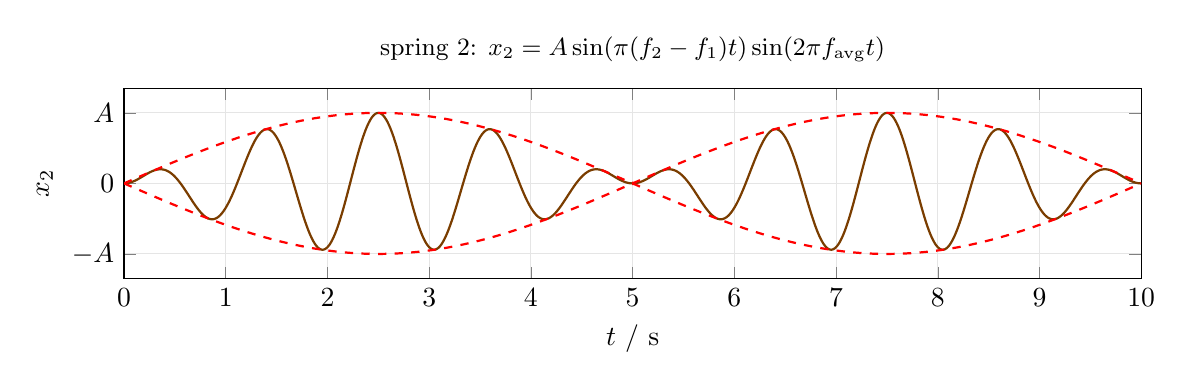
\begin{tikzpicture}
\begin{axis}[width=14.5cm,height=4.0cm,xlabel={$t$ / s},ylabel={$x_2$},xmin=0,xmax=10,ymin=-1.35,ymax=1.35,ytick={-1,0,1},yticklabels={$-A$,$0$,$A$},grid=major,grid style={gray!20},title={\small spring 2: $x_2=A\sin(\pi(f_2-f_1)t)\sin(2\pi f_{\rm avg}t)$}]
\addplot[thick,copper!60!black,domain=0:10,samples=700]{sin(deg(0.2*pi*x))*sin(deg(1.8*pi*x))};
\addplot[thick,red,dashed,domain=0:10,samples=300]{abs(sin(deg(0.2*pi*x)))};
\addplot[thick,red,dashed,domain=0:10,samples=300]{-abs(sin(deg(0.2*pi*x)))};
\end{axis}
\end{tikzpicture}
\caption{Beats for equal mode amplitudes. Top: the released spring and its envelope (red dashed); the swellings recur every $T_{\rm beat}=1/(f_2-f_1)$, and the fast oscillation has period $1/f_{\rm avg}$. Bottom: spring~2 carries the same two frequencies with the anti-phase term reversed, $x_2=\frac A2(\cos\omega_1t-\cos\omega_2t)=A\sin(\pi(f_2-f_1)t)\sin(2\pi f_{\rm avg}t)$; its envelope is a quarter of a beat behind, so it swings most when spring~1 is momentarily still. This is the energy transfer between the springs.}
\label{fig:beatplot}
\end{figure}

\subsubsection{Spring 2, and a test of identical springs}

Spring~2 contains the same two cosines with the sign of the anti-phase term reversed (equation~\eqref{eq:solution}). Hence (i) its spectrum has peaks at the same $f_1$ and $f_2$; (ii) for identical springs the height ratio $\xi_0/\eta_0$ is the \emph{same} for both springs whatever the starting condition, because each mode has equal amplitude in both springs (mode shapes $(1,1)$ and $(1,-1)$); (iii) if the springs are not identical the mode shapes tilt and the two ratios differ, so comparing them is a direct test of the identical-spring assumption (used in the evaluation).

\subsubsection{Predictions for the average and beat frequencies}

Combining $f_2=\sqrt{f_1^2+Cd^{-5}}$ from \eqref{eq:main} with the definitions,
\begin{equation}
f_{\rm beat}=\sqrt{f_1^2+Cd^{-5}}-f_1=\frac{Cd^{-5}}{2f_{\rm avg}},\qquad
f_{\rm avg}=\frac{f_1+\sqrt{f_1^2+Cd^{-5}}}{2}.
\label{eq:favg_fbeat}
\end{equation}
Because $f_{\rm avg}$ can only vary between $f_1$ (weak coupling) and about $1.15f_1$ (closest separation used), while $d^{-5}$ varies by a factor of $25$ over the range, the beat frequency falls almost as steeply as $d^{-5}$ itself---for weak coupling $f_{\rm beat}\approx Cd^{-5}/2f_1$ exactly follows the inverse-fifth-power law---while the average frequency is nearly constant and rises above $f_1$ only where the coupling is strong. Numerically, the beat period should lengthen from about $4\un{s}$ at $21\un{mm}$ to over $100\un{s}$ at $40\un{mm}$ and to some ten minutes at $60\un{mm}$; this is why no second peak can be resolved at the largest separations in a $30\un{s}$ record.

% ============================================================================
\subsection{Assumptions}\label{sec:assumptions}

The derivation assumed:
\begin{enumerate}[label=(\alph*),nosep,leftmargin=2em]
\item the magnets are point dipoles ($d\gg D$) --- entered in \eqref{eq:F};
\item the displacements are small enough for the force to be linearised ($A\ll d$) --- entered in \eqref{eq:taylor};
\item the two springs are identical ($k$ and $m$ the same for both) --- needed for the decoupling in \eqref{eq:modes};
\item each spring can be represented by a single lumped mass --- \eqref{eq:meff};
\item there is no damping;
\item the magnets stay coaxial (the tip of a bending cantilever actually tilts slightly) --- \eqref{eq:Baxis};
\item the FFT returns the true frequencies of the motion.
\end{enumerate}
Each is revisited in the evaluation, where its sign, size and remedy are estimated.

\begin{table}[htbp]
\centering\footnotesize
\caption{Symbols used in this section.}
\label{tab:symbols}
\begin{tabular}{@{}p{2.8cm}p{4.0cm}p{3.2cm}p{4.6cm}@{}}
\toprule
Symbol & Meaning & Symbol & Meaning\\
\midrule
$L,\ b,\ h$ & free length, width, thickness of a strip & $d$ & equilibrium centre-to-centre separation of the magnets\\
$s,\ y(s)$ & distance along the strip from the clamp; sideways deflection there & $d_0$ & spacing of the clamps ($d=d_0+2\delta$)\\
$E$ & Young's modulus of copper & $\delta$ & static outward bend of each spring, $k\delta=F(d)$\\
$I=bh^3/12$ & second moment of area of the cross-section & $x_1,\ x_2$ & displacements of the magnets from equilibrium (both positive to the right)\\
$\mathcal M(s)$, $R$ & bending moment; radius of curvature & $u=x_2-x_1$, $r=d+u$ & change of separation; instantaneous separation\\
$k=3EI/L^3$ & tip stiffness of a spring & $\gamma=-F'(d)$ & magnetic stiffness $=6\muz\mum^2/\pi d^5$\\
$\varphi(s)$ & normalised deflection curve, eq.~\eqref{eq:phi} & $\eta=x_1+x_2$, $\xi=x_1-x_2$ & normal coordinates\\
$M,\ \mu$ & magnet mass; strip mass per unit length & $\omega_1,\ \omega_2$; $f_1,\ f_2$ & angular / ordinary frequencies of the in-phase and anti-phase modes\\
$m=M+\frac{33}{140}\mu L$ & effective oscillating mass & $\eta_0,\ \xi_0$ & mode amplitudes, eq.~\eqref{eq:amps}\\
$\mum$, $\muz$ & dipole moment of a magnet; permeability of free space & $A$, $x_{20}$ & release displacement of spring 1; shift of spring 2 while spring 1 is held\\
$B(r)$, $U(r)$, $F(r)$ & on-axis field, energy, repulsive force & $C=3\muz\mum^2/\pi^3m$ & constant in $f_2^2-f_1^2=Cd^{-5}$\\
& & $f_{\rm avg}$, $f_{\rm beat}$, $T_{\rm beat}$ & $(f_1+f_2)/2$; $f_2-f_1$; $1/f_{\rm beat}$\\
\bottomrule
\end{tabular}
\end{table}

\end{document}
